\section{问题三：全向干扰源的搜索、定位与清除}
\label{new:sec-q3}

\subsection{任务特点与总体思路}
问题三中的干扰源均为全向发射源。机器人在检测点收到信号，便可据此把该频道的源位置限制在一个保守可行域内；对尚未发现的频道，若在一个覆盖保证为1000米的检测点未收到信号，则真源必满足\(\norm{g-s}>1000\)米。因而本问在扫描与定位之间采用边发现、边调度：一旦某频道出现正观测，立即插入该频道的定位任务，同时继续保留尚未履行的七点扫描义务。搜索、定位和清除三阶段使用同一频道状态，避免把“已经发现”误当成“已经完成”。

设源区域为
\[
 \disk=\{g\in\mathbb R^2:\norm g\le R\},\qquad R=1800\ \mathrm m,
\]
题给最小接收半径为$1000$米，最大接收半径为$1500$米。本文把七点环作为问题三的基准发现骨架，采用环半径$d=1200$米；随后按照当前位置与任务代理点的距离统一安排检测任务，问题三取代理目标中的$\gamma=0$。这一构造是完整覆盖下的可执行方案，不把七点下界误读为允许半径1000米时任意布局的全局最优性结论。区域覆盖与路径规划的相关研究同样强调覆盖完整性和路径代价的协同权衡\cite{ren,jia}。

\subsection{七点环构造与覆盖半径}
取原点及正六边形环上的六个检测点：
\begin{equation}
 p_0=(0,0),\qquad p_{k+1}=d\,u(k\pi/3),\quad k=0,\ldots,5,
 \qquad u(\theta)=(\cos\theta,\sin\theta).
 \label{new:eq-seven-points}
\end{equation}
七个位置同时承担每个频道的发现义务。令$g=r u(\theta)$。总有一个环点与$g$的极角差不超过$\pi/6$，因此在固定半径$r$的圆周上，到最近检测点的最坏距离为
\begin{equation}
 f_d(r)=\min\left\{r,\sqrt{r^2+d^2-\sqrt3dr}\right\}.
 \label{new:eq-ring-envelope}
\end{equation}
第一项对应原点，第二项对应相邻环点的角平分线。两项在$r=d/\sqrt3$处相等；在此之前原点更近，在此之后环点更近。后一项的平方是$r$的凸二次函数，所以在区间端点达到最大值。在参数范围$1200\le d\le900\sqrt3$内，七点构型的精确覆盖半径为
\begin{equation}
 \rho(d)=\max_{g\in\disk}\min_{0\le j\le6}\norm{g-p_j}
 =\max\left\{\frac d{\sqrt3},
 \sqrt{R^2+d^2-\sqrt3Rd}\right\}.
 \label{new:eq-ring-radius}
\end{equation}
这个证明覆盖了圆盘内部、外边界以及六个扇区的接缝，不依赖网格采样。$d=900\sqrt3$时两项均为$900$米，给出传统的900米覆盖基线。

当$d=1200$米时，边界项控制最坏距离：
\begin{equation}
\begin{aligned}
 \rho(1200)&=\sqrt{1800^2+1200^2-\sqrt3\cdot1800\cdot1200}\\
 &\approx968.901572\ \mathrm m,\\
 1000-\rho(1200)&\approx31.098428\ \mathrm m.
\end{aligned}
 \label{new:eq-ring-margin}
\end{equation}
因此在理想点位下，七点环距离题给最小接收半径仍有约$31.10$米余量。若理想点与实际停靠点的总欧氏偏差不超过$\eta$，由三角不等式，实际最坏距离不超过$\rho(1200)+\eta$；例如$\eta\le1$米时仍严格小于1000米。这里的余量只说明全向发现骨架的距离鲁棒性，并不等同于测向角误差或局部清除半径。

900米半径下七点的必要性也可作简洁说明。距原点为$t$的一个半径900米圆盘，在源圆周上能够覆盖的交弧半宽$\beta$满足
\[
 \cos\beta=\frac{R^2+t^2-900^2}{2Rt}
 \ge\frac{\sqrt{R^2-900^2}}R=\cos(\pi/6).
\]
故每个非中心圆盘的弧宽至多为$\pi/3$，覆盖整条边界至少需要六个，并且等号迫使六个圆心位于半径$900\sqrt3$的正六边形环上；这些圆盘又不能覆盖原点，所以还必须增加中心点。这个下界仅针对900米覆盖要求。允许半径改为1000米后，弧宽约束改变，本文不声称七点是所有布局的全局最优。

\subsection{骨架路径与联合调度}
从原点出发依次访问六个环点，环上相邻点弦长为$d$，任意两个不同环点的距离不小于$d$。因此开放骨架路径的最短长度为
\begin{equation}
 L_{\rm ring}^{\min}(d)=6d.
 \label{new:eq-ring-path}
\end{equation}
沿环依次访问即可达到该下界；插入中间停靠点不能缩短折线。最终$d=1200$米时，纯骨架长度为7200米。这个数值不包含定位支线、清除动作和频道切换，不能直接当作每局实际节省时间。

执行时，不把七个检测点孤立地排成一条预先固定的路线。设当前位置为$q$，每一个未完成骨架点或已发现未清除频道都形成一个任务代理。骨架任务的代理半径为0；已知频道以其当前保守域最小包围圆中心$z_c$及半径$r_c$表示。对任务排列$\pi$，采用开放路线代理目标
\begin{equation}
 J_\gamma(\pi)=\norm{q-z_{\pi_1}}+
 \sum_{j=1}^{n-1}\norm{z_{\pi_{j+1}}-z_{\pi_j}}+\gamma r_{\pi_1}.
 \label{new:eq-route-proxy}
\end{equation}
问题三的基准 refined 联合调度取$\gamma=0$，即只按几何行程安排首个任务，不对首个不确定区域另加半径惩罚。该目标只是排序代理，不替代真实的测量、定位和清除耗时。

算法先以最近插入法形成完整任务排列，再进行有界的连续区间反转改进。每次只执行当前排列首项；动作完成后，根据新的位置、频道状态和观测结果重建任务集。骨架任务与频道任务即使坐标重合也不合并，以确保所有七个覆盖义务均被实际履行。这样，联合调度只改变访问次序，不删去任何用于认证未知频道的检测位置。2-opt作为旅行商路径的局部搜索操作已有相关算法研究\cite{wang}。

\subsection{局部测向与清除}
在七点扫描得到正观测后，记录该频道的测向角，并以初始位置圆盘与各次测向约束的交集作为保守可行域$P_c$。每次测向的角度误差按题设和实现的保守边界扩张半平面；因此真实源始终满足
\begin{equation}
 g_c\in P_c.
 \label{new:eq-q3-invariant}
\end{equation}
问题三的局部定位最多使用6次固定测向。每次测量均从当前可行域和已拒绝位置出发选择新的接入点；基准 refined 收到\texttt{direction}后加入相应的角度约束，收到\texttt{no\_signal}则保留原可行域并记录失败探测，不能把失败位置当作新的正约束。field在问题三对有效无信号进一步使用下述保守外包。收到\texttt{near}时进入原有的清除流程。

记当前最小包围圆为$B(z,r)$，机器人位置为$q$。每一轮先检查清除条件：若$q$到$P_c$全部顶点的距离不超过19.9米，则原地清除；若$r\le19.9$米，则到$z$清除。若$19.9<r\le38$米，先在中心作一次预测清除；这种尝试不具有全域保证，失败后立即转入完整光学覆盖，不反复测向。阈值38米用于在有限观测与光学搜索之间切换，而19.9米才是保守清除条件。

对更大的区域，取最近一个收到正示向的位置$s^+$，令$e=(z-s^+)/\norm{z-s^+}$、$n=(-e_2,e_1)$，沿示向法向构造左右两个候选点
\[
 p_\pm=z\pm\delta n,\qquad
 \delta=\min\{120,\max\{25,0.22r\}\}\ \mathrm m.
\]
从尚未失败的候选点中选择较近者测向；该横向偏移使新的示向线与原示向线形成交角，有助于压缩长条形可行域。最多6次测向用完，或发生无法继续选点的退化情形时，转入完整光学覆盖。每次调用局部过程均以该频道成功清除为正常返回条件；若观测不一致或完整覆盖仍未清除，则报告异常并中止，不能以未清除状态返回调度后重新获得六次预算。

清除判定使用半径$19.9$米的保守覆盖，而不是把直径小于40米简单当作半径20米证书。若当前凸多边形的全部顶点都落入以计划清除点$a$为中心、半径$19.9$米的圆盘，则由凸性有$P_c\subseteq B(a,19.9)$，结合式\eqref{new:eq-q3-invariant}可知真源距$a$不超过设备的20米清除半径，并留有0.1米余量。默认 refined 不启用沿射线缩短接入的 approach；该动作只属于下述 field 对照增强。几何上满足条件不等于已经清除，只有接口返回该频道的\texttt{success}才可更新为完成。
作为对照增强，field 版本还可在满足条件时做一次原地预检测，并在问题三使用负观测的保守凸外包：将严格位于1000米圆盘内部的正十六边形各边外侧保留，再取保留片的凸包。对全向源，\texttt{no\_signal}排除的是该1000米接收圆盘内部的真源位置；但该外包只是效率层的保守收缩，不能改变七点扫描义务。安全近侧清除同样只缩短已经由当前可行域保证的接入段。上述两项属于对照增强，不改变本文默认的 refined 基准。

当局部测向达到上限仍有$r>19.9$米时，采用矩形网格覆盖整个$P_c$，而非只覆盖其顶点。取当前可行域直径方向为正交坐标轴，令包围矩形为$[x_-,x_+]\times[y_-,y_+]$，并取安全半径$\bar r=19.9-\varepsilon$。令
\[
 h=\sqrt2\,\bar r,\qquad
 N_x=\max\!\left(1,\left\lceil\frac{x_+-x_-}{h}\right\rceil\right),\quad
 N_y=\max\!\left(1,\left\lceil\frac{y_+-y_-}{h}\right\rceil\right),
\]
将矩形分成$N_xN_y$个小矩形，在第$(i,j)$格中心
\[
 a_{ij}=\left(x_-+\frac{i+1/2}{N_x}(x_+-x_-),\\
 y_-+\frac{j+1/2}{N_y}(y_+-y_-)\right)
\]
执行光学检测。每个小矩形的两边均不超过$h$，故任意$w$落在该格内时
\[
 \norm{w-a_{ij}}\le\frac12\sqrt{h^2+h^2}=\bar r<19.9.
 \]
\begin{equation}\label{eq:optcover}
 P_c\subseteq\bigcup_{i=0}^{N_x-1}\bigcup_{j=0}^{N_y-1}B(a_{ij},19.9).
\end{equation}
包围矩形覆盖$P_c$，所以这些圆盘覆盖$P_c$的每一个点；真源属于$P_c$，必被至少一个光学点覆盖。最后仍须以接口返回的\texttt{success}作为清除证书。$\varepsilon$只吸收坐标舍入和边界浮点余量，不改变19.9米阈值。
\begin{figure}[htbp]
 \centering
 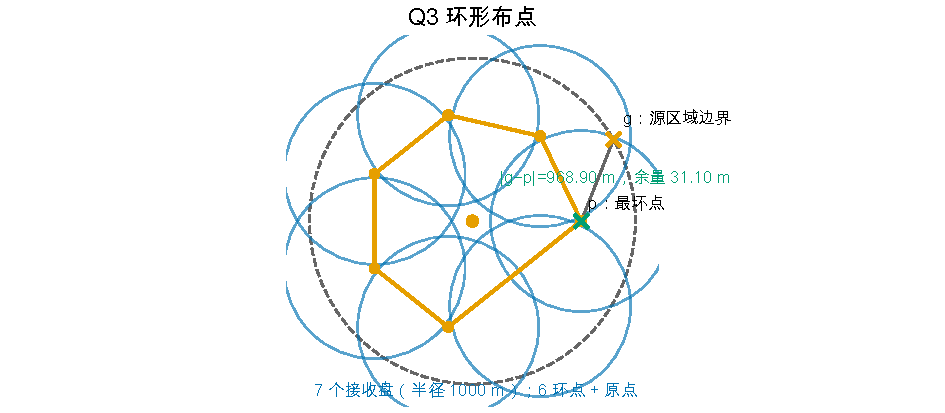
\includegraphics[width=0.78\textwidth]{figures/competition_ring.pdf}
 \caption{问题三七点环发现骨架。圆盘为半径1800米的源域，环半径取1200米；图中几何位置为示意，实际机器人停靠误差由覆盖余量吸收。}
 \label{new:fig-q3-ring}
\end{figure}

\begin{figure}[htbp]
 \centering
 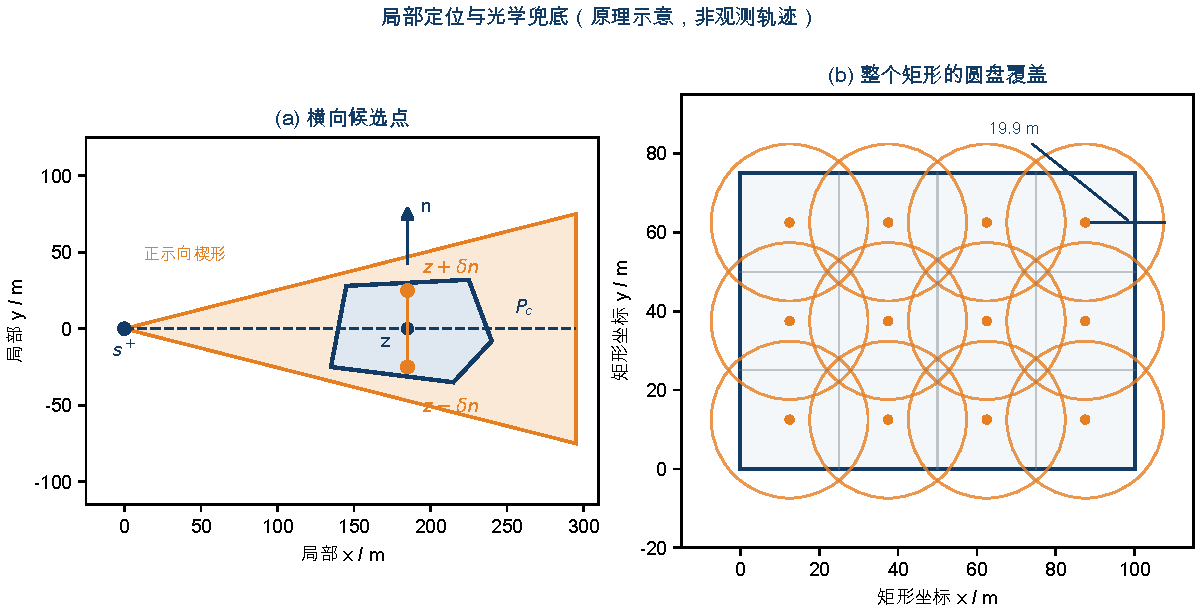
\includegraphics[width=0.82\textwidth]{figures/competition_localize.pdf}
 \caption{局部测向与光学覆盖示意。正观测逐步收缩保守可行域，最终以矩形覆盖并逐顶点验证19.9米清除条件；示意线段不表示观测轨迹。}
 \label{new:fig-q3-localize}
\end{figure}

\subsection{扫描规则与逐频道停止条件}
未知频道必须在七个骨架位置逐一检测。已建立正测向轨迹但尚未清除的频道，不因骨架点再次无信号而被判定为无源，而是保留为独立的定位清除任务；这一区分避免把已知源从扫描记录中错误删除。已知频道收到的负观测不填入未知频道的完成集合，也不替代清除反馈。

对每个频道$c$定义完成证书
\begin{equation}
\operatorname{Cert}_c=
\begin{cases}
 C,&\text{已收到频道$c$的\texttt{success}清除反馈},\\
 N,&\text{从未发现该频道源，且七个位置均得到有效无信号},\\
 U\text{或}D,&\text{尚未确定，或已发现但未清除}.
\end{cases}
 \label{new:eq-stop-certificate}
\end{equation}
只有在全部20个频道均取得$C$或$N$证书，或者已经收到16个不同频道的$C$证书时，任务才可停止：
\begin{equation}
 \left[\forall c\in\{1,\ldots,20\},\ \operatorname{Cert}_c\in\{C,N\}\right]
 \quad\text{或}\quad
 \left[\#\{c:\operatorname{Cert}_c=C\}=16\right].
 \label{new:eq-stop}
\end{equation}

式\eqref{new:eq-stop}中的第二种情形使用题给源数上界，统计的是不同频道的成功清除数，而不是清除尝试数。队列暂时为空、连续无信号、或动作异常都不能替代证书。由于全向覆盖定理保证未知频道的真源若存在必落入至少一个有效接收圆盘，七点扫描全部无信号时才可形成$N$证书；一旦频道进入$D$状态，则必须以$C$完成，不能再转为$N$。

\subsection{算法流程与结果说明}
问题三的实施步骤为：
\begin{enumerate}
 \item 初始化20个频道状态与七点骨架任务，当前位置设为原点；
 \item 按$J_0$对未完成骨架任务和已知未清除频道统一排序，执行最近插入及有界2-opt得到开放路线；
 \item 对当前首项执行真实测量或清除动作。未知频道不跳过骨架位置，已知频道仅作为定位清除任务调度；
 \item 对正观测维护保守凸可行域，最多进行6次局部测向，随后进行矩形光学覆盖和清除尝试；
 \item 仅在收到\texttt{success}后记为$C$；未发现频道在全部七点有效无信号后记为$N$；
 \item 重建任务集并重复，直至满足式\eqref{new:eq-stop}。
\end{enumerate}

结果评价统一按实际执行的移动距离、测量次数、换频次数、清除尝试及动作时间计算。七点构造提供全域发现保证，联合调度减少的是任务间的无效绕行，而不是检测义务；局部测向和矩形光学覆盖保证的是已发现频道的清除路径。Q3官方演练的全清结果和局均时间在模型检验章中统一列示，局部测向、光学覆盖与路线机制的分项结果也在该章进行比较。基准 refined 与 field 对照增强分开统计，以区分几何覆盖构造与效率调度的作用。
